\documentclass[preview]{standalone}
\usepackage[all]{genealogytree}
\usetikzlibrary{decorations}
\usetikzlibrary{positioning}
\usetikzlibrary{decorations.pathreplacing}
\tcbuselibrary{listings}

\newcommand{\internalnodes}[2][magenta, green]{
			% box={underlay={\begin{tcbclipinterior}
            %     \fill[#1] ([xshift=-3mm] interior.center) circle (1mm);
            %     \fill[#2] ([xshift=3mm] interior.center) circle (1mm);
            % \end{tcbclipinterior}}}
        }
\begin{document}

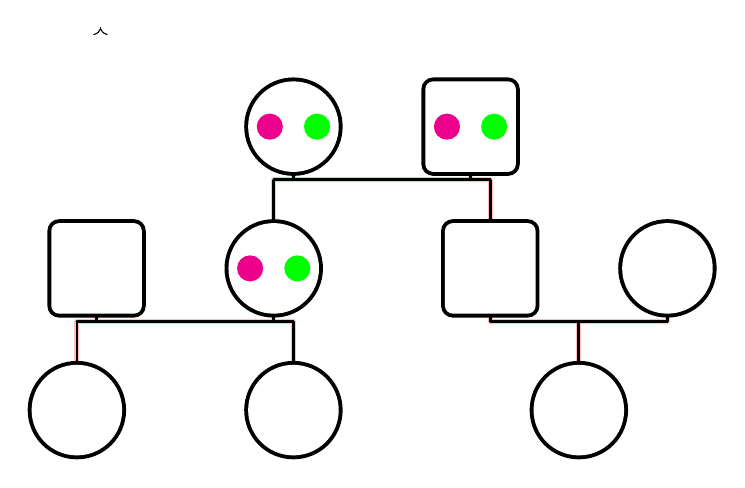
\begin{tikzpicture}
    \genealogytree[
        template=formal graph,
        tcbset={male/.style={colback=white,colframe=black,width=1.25cm,height=1.25cm},
        female/.style={circular arc,colback=white,colframe=black,width=1.25cm, height=1.25cm}},
        edges={anchoring=center,foreground=black,background=pink},
        level distance=1cm,
        parent distance in child graph=1cm,
        child distance in child graph=1.5cm
        ]{
        child[id=gparental]{
        g[id=gma,female,
			 box={underlay={\begin{tcbclipinterior}
				 \node[circle,fill=magenta](gma1) at ([xshift=-3mm]interior.center){};
				 \node[circle,fill=green](gma2) at ([xshift=3mm]interior.center){};
             \end{tcbclipinterior}}}]
        {}
        p[id=gpa,male,
			 box={underlay={\begin{tcbclipinterior}
				 \node[circle,fill=magenta](gpa1) at ([xshift=-3mm]interior.center){};
				 \node[circle,fill=green](gpa2) at ([xshift=3mm]interior.center){};
             \end{tcbclipinterior}}}]
        {}
        child[id=parental] {
            p[id=dad,male]{}
            c[id=sib,female]{}
            c[id=you,female]{}
            g[id=mom,female,
			 box={underlay={\begin{tcbclipinterior}
				 \node[circle,fill=magenta](mom1) at ([xshift=-3mm]interior.center){};
				 \node[circle,fill=green](mom2) at ([xshift=3mm]interior.center){};
             \end{tcbclipinterior}}}]
            {}
        }
        child[id=cousins]{
        g[id=uncle,male]{}
        c[id=cousin,female]{}
        p[id=aunt,female]{}
        }
    }
    }
    \draw[->, black] (gpa2.center) --  (mom2.center);
    % \draw[->, pink] ([xshift=3mm] gma.center) --  ([xshift=-3mm] mom.center);
    % \node[] at (gpa) {Poop};
\end{tikzpicture}

\end{document}




